%%%%%%%%%%%%%%%%%%%%%%%%%%%%%%%%%%%%%%%%%%%%%%%%%%%
%
%  New template code for TAMU Theses and Dissertations starting Fall 2016.  
%
%
%  Author: Sean Zachary Roberson
%  Version 3.17.09
%  Last Updated: 9/21/2017
%
%%%%%%%%%%%%%%%%%%%%%%%%%%%%%%%%%%%%%%%%%%%%%%%%%%%
%%%%%%%%%%%%%%%%%%%%%%%%%%%%%%%%%%%%%%%%%%%%%%%%%%%%%%%%%%%%%%%%%%%%%%
%%                           SECTION III
%%%%%%%%%%%%%%%%%%%%%%%%%%%%%%%%%%%%%%%%%%%%%%%%%%%%%%%%%%%%%%%%%%%%%



\chapter{RESULTS*}


%% \begin{prop}
%% The action of the mapping class group on the vector space $H$ induced by the action of the orientation-preserving homeomorphisms on the surface $\Si$ is well-defined.
%% \end{prop}
%% \begin{proof}
%% The orientation-preserving group $\Homeo^+(M)$ acts on colored embedded graphs in $\Si$.  To see that the mapping class group $\MCG(\Si)$ has a well-defined action on $H$, we need to check two things: first, that isotopic homeomorphisms acting on a colored graph take it to equivalent colored graphs and, second, that a homeomorphism maps equivalent colored graphs to equivalent colored graphs.

%% For the first, suppose $f, g \in Homeo^+(M)$ are isotopic, with $H: M \times I \to M$ an isotopy from $f$ to $g$.  Let $i: \Gamma \to M$ be an graph embedding.  Then $H \circ i$ is an isotopy from $f \circ i$ to $g \circ i$.    

%% For the second,  to check that a homeomorphism $f \in \Homeo^+(M)$ preserves equivalence of colored graphs, it suffices to check that it in the case of each local move.  Since the mapping class group is generated by Dehn twists, all the local moves reduce to the isotopy move. 

%% To check that isotopic colored graphs get mapped to equivalent colored graphs, suppose $\Gamma$ is a graph and $i: \Gamma to M$ and $j: \Gamma \to M$ are isotopic embeddings. Let $H: \Gamma \times I \to M$ be an isotopy from $i$ to $j$.  Let $f \in \Homeo^+(M)$.  Then $f \circ H$ is an isotopy from $f \circ i$ to $f \circ j$.  

%% Thus, the action of the mapping class group on $H$ is well-defined.
%% \end{proof}

%% TODO: Prove that the Turaev-Viro/ RT construction gives the same thing for equivalent TQFTs

\newcommand{\B}{\mathcal B}

%% \begin{prop} \label{prop:equivCats}
%% Let $\Sigma$ be a compact surface with boundary. Let $\mathcal A$ and $\mathcal B$ be monoidally equivalent spherical fusion categories.  Then
%% the TVBW-representation $\rho_A : \MCG(\Sigma) \to GL(H_A)$ associated to $\mathcal A$ is isomorphic to the representation associated to $\mathcal B$.
%% \end{prop}
%% \begin{proof}
%% Let $(F, J)$ be a monoidal equivalence from $\A$ to $\B$. I claim that $F$ induces an isomorphism $\overline{F}: H_A \to H_B$ by acting on the labels.  To see that this is well-defined, we need to check that if $\phi \in \Hom(\one, V_1 \otimes \cdot \otimes V_n)$ then $F(\phi) \in    \Hom(\one, F(V_1) \otimes \cdot \otimes F(V_n))$


%% To see this, we need to check that $F$ preserves the local relations.  For the first local relation (contracting an edge), we need to check that $F(\ev_{F(X)}) \circ (F(\phi) \otimes F(\psi)) = F(\ev_{F(X)} \circ (\phi \otimes \psi))$.
%% \end{proof}


To show that the image of any $\Vect_G^\omega$ mapping class group representation is finite, we will analyze the action of the mapping class group on a finite collection of colored graphs that span the representation space $H$.  To define this spanning set, we will need the following definitions of simple morphisms and colored graphs. \let\thefootnote\relax\footnote{* Reprinted with permission from ``Finiteness for mapping class group representations from twisted dijkgraaf--witten theory,'' P.\ P.\ Gustafson, \emph{Journal of Knot Theory and Its Ramifications}, vol. 27, no. 06, p. 1850043, Copyright 2018 by World Scientific Publishing Company.}


\begin{defn} \label{def:simple_morphism}
  Let $g_1, \ldots, g_n \in G$ and $\epsilon_1, \ldots, \epsilon_n  \in \{\pm 1\} = \ZZ_2$.  A morphism
  \begin{align*}
    \phi \in \langle (\delta_{g_1}, \epsilon_1), \ldots, (\delta_{g_n}, \epsilon_n) \rangle & = \Hom_{\widehat{\vgo}}(1, (\delta_{g_1}, \epsilon_1) \otimes \cdots \otimes (\delta_{g_n}, \epsilon_n)) \\
    & = \Hom_{\vgo}(1, (( \cdots ((\delta_{g_1^{\epsilon_1}} \otimes \delta_{g_2^{\epsilon_2}}) \otimes \cdots  \otimes \delta_{g_n^{\epsilon_n}})
  \end{align*}
  will be called \emph{simple} if it is the composition of the isomorphism $\one \cong \delta_1$ and  tensor product isomorphisms of the form $\delta_{gh} \cong \delta_g \otimes \delta_h$ in $\vgo$.
\end{defn}

By MacLane's coherence theorem applied to the $\vgo$ Hom-space, there is a unique simple morphism in $\langle (\delta_{g_1}, \epsilon_1), \ldots, (\delta_{g_n}, \epsilon_n) \rangle$ whenever $\prod_{i=1}^n g_i = 1$. This simple morphism is a canonical basis element for the 1-dimensional space $\langle (\delta_{g_1}, \epsilon_1), \ldots, (\delta_{g_n}, \epsilon_n) \rangle$.  We will describe a map between such spaces as multiplication by a scalar, where the scalar is the matrix coefficient of the map with respect to these canonical bases.

\begin{defn} \label{def:simple_graph}
Let $\Gamma$ be a graph embedded in a surface $\Si$.  A $\widehat {\Vect_G^\omega}$-coloring $(V, \phi)$ of $\Gamma$ will be called \emph{simple} if the following conditions both hold: 
\begin{enumerate}
\item For every oriented edge $\ee \in E^{or}(\Gamma)$, there exists a group element $g(\ee) \in G$ and $\epsilon(\ee) \in \{\pm 1\} = \ZZ_2$ such that the coloring $V(\ee) = (\delta_{g(\ee)}, \epsilon(\ee))$.
\item If $v$ is an interior vertex of $\Gamma$, then there exists an enumeration  $\ee_1, \dots, \ee_n$ of the edges incident to $v$, taken in counterclockwise order and with outward orientation, such that $\prod_{i=1}^n g(\ee_i)^{\epsilon(\ee_i)} = 1$ and  the vertex label $\phi(v) \in \langle g(\ee_1), \ldots, g(\ee_n) \rangle$ is a simple morphism.
\end{enumerate}
\end{defn}


\begin{lem} \label{lem:z_simple}
Let $\phi \in \langle (g_1, \epsilon_1), \ldots, (g_n, \epsilon_n) \rangle$ and $\psi \in \langle (g_n, \epsilon_n), (g_1, \epsilon_1), \ldots, (g_{n-1}, \epsilon_{n-1}) \rangle$ be simple morphisms.  Then $z(\phi) = \alpha \psi$, where $\alpha \in \mu_{|G|}$.
\end{lem}
\begin{proof}
The definition of the $z$-morphism in Equation \ref{e:cyclic} only involves tensors and compositions of structural morphisms of $\widehat \vgo$, which are equal to tensors and compositions of identities, associators, unitors, the pivotal $j$-morphism, evaluation, and coevaluation morphisms in $\vgo$ on the corresponding objects.  Since all the tensor factors in the codomain of $\phi$ are of the form $(\delta_g, \epsilon)$ for some $g \in G$ and $\epsilon \in \ZZ_2$, the definition of $\Vect_G^\omega$ implies that each of the structural morphisms simply consist of multiplication by elements of the form $\omega(g,h,k)$ for some $g,h,k \in G$. Thus, $z(\phi) = \alpha \psi$ for some $\alpha$ which is a product of elements in $\Img(\omega)$.   Since $\Img(\omega) \subset \mu_{|G|}$, it follows that $\alpha \in \mu_{|G|}$.
\end{proof}

\begin{prop} \label{prop:omega}
Let $\Gamma$ be a simple colored graph embedded in a surface $\Sigma$.  Let $\Delta$ be the colored graph given by applying one of the three local moves in Figure \ref{f:local_rels1} to $\Gamma$.  Then there exists $\alpha \in \mu_{|G|}$ such that $$\Delta - \alpha \Delta' \in N(\Sigma, \VV),$$
where $\Delta'$ is a simple colored graph given by replacing each vertex label in $\Delta$ with a simple morphism and each edge label by a object of the form $(\delta_g, \epsilon)$ for some $g \in G$ and $\epsilon \in \ZZ_2$.
\end{prop}
\begin{proof}
We'll consider each local move separately.  In each case, we need to show that $\Delta$ is equivalent to $\alpha \Delta'$ in $H$.  

For the first (edge contraction) local move in Figure \ref{f:local_rels1},  using the same notation as in the figure, the vertex label $\psi \cc{X} \phi$ in $\Delta$ is given by the following composition in $\vgo$ (recall that every $\widehat \vgo$ Hom-space is equal to a $\vgo$ Hom-space).  Since $\Gamma$ is simple, there exist integers $l,k$ and simple morphisms $\phi', \psi'$ such that $\psi = z^l(\psi')$ and $\phi = z^k(\phi')$. Then we repeatedly apply associators and the cyclic $z$-morphism of Equation \ref{e:cyclic} to $\phi$ and $\psi$ until the tensor factors of the codomain are rearranged in the order of the left hand side of Equation \ref{e:composition} and that $X$ and $X^*$ are isolated (not contained in any parentheses).  After applying the $\ev_X$ morphism, we reassociate until the new label $\ph\cc{X}\psi$ has the left-associated parenthesization.  Since every edge is labeled by a $(\delta_g, \epsilon)$ for some $g \in G$ and $\epsilon \in \ZZ_2)$, each associator morphism consists of multiplication by $\omega(g,h,k)$ for some $g,h,k \in G$.  Similarly, by Lemma \ref{lem:z_simple}, every $z$-morphism consists of multiplication by some $\beta \in \mu_{|G|}$.  Thus, the overall composition consists of multiplication by an element $\alpha \in \mu_{|G|}$.

For the second local move (tensoring parallel edges), there are two cases: $k = 0$ and $k > 0$.  In the $k = 0$ case,  we apply inverse unitors to each vertex label to introduce an edge labeled by the unit object, followed by reassocation.  In the $k > 0$ case, tensoring in $\widehat \vgo$ corresponds to applying associators and tensor product isomorphisms in $\vgo$ Hom-spaces.  Since every edge is labeled by a simple object, it follows that the result of this local move is also of the desired form.

For the third local move (adding a $\coev$-labeled vertex), the colored graph given by direct application of the local move to a simple graph has an extra vertex labeled by $\coev_{\delta_g}$ in $\widehat \vgo$ for some $g \in G$, which is a simple morphism by definition.  
\end{proof}


\section{No Boundary Case}

We first prove our theorem in the easier case where the surface $\Si$ is closed.  

\begin{thrm}\label{thm:closed}
The image of any twisted Dijkgraaf-Witten representation of a mapping class group of an orientable, closed surface $\Si$ is finite.
\end{thrm}

\begin{proof}
Let $\Gamma$ be a $\widehat \vgo$-colored graph embedded in $\Si$, and let $g \ge 1$ be the genus of $\Si$ (if $g = 0$, the mapping class group is trivial). Thinking of $\Si$ as a quotient of its fundamental $4g$-gon, by isotopy we may assume that the vertices of $\Gamma$ lie in the interior of the polygon, none of the edges of $\Gamma$ intersect the corners of the polygon, and that the edges of $\Gamma$ only meet the sides of the polygon transversally.  Applying the evaluation map of Theorem \ref{t:RT} on the interior of the polygon shows that $\Gamma$ is equivalent to a graph with a single vertex whose edges are simple closed curves, each of which intersect the boundary of the polygon precisely once.  By using the local relations, we can replace all the edges intersecting a side with a single edge labeled by the tensor product of their labels.  If there are no edges intersecting a side, we can insert a single edge labeled by the group identity into $\Gamma$ that intersects only that side.  Thus, $\Gamma$ is equivalent to a colored graph with one vertex $v$ and edges $e_1, \ldots, e_{2g}$ corresponding to the standard generators of $\pi_1(M,v)$ as shown in Figure \ref{fig:span}.

By Theorem \ref{t:RT} and the definition of the quotient map identifying the sides of the fundamental polygon, the vertex $v$ is colored by an element $\phi(v) \in \Hom (\one, \bigotimes_{i=1}^g V(e_{2i-1}) \otimes V(e_{2i})  \otimes V(e_{2i-1})^* \otimes V(e_{2i})^*)$, where $V(e_i) \in \Obj \widehat \vgo$ is the coloring of the edge $e_i$.   

We claim that the representation space $H$ is spanned by the set of such colored graphs $\Gamma$ such that each $V(e_i)$ is simple. This follows from the additivity of the evaluation map of Theorem \ref{t:RT} in the direct sum.   Strictly speaking, we can only take advantage of the additivity on a disk, not on an edge $e_i$, which is a $v$-based loop. However, we can easily add a $\coev$-labeled vertex to any edge $e_i$, apply the additivity on one of the two resulting edges (which lies in an embedded disk), and then contract on the other edge to get the decomposition we want.

Since isomorphic colorings give the same evaluation, it follows that $H$ is spanned by colored graphs $\Gamma$ such that
each $V(e_i) = \delta_{g_i}$ for some $g_i \in G$.  For such $\Gamma$,  the space of possible $v$-colors $\Hom (\one, \bigotimes_{i=1}^g V(e_{2i-1}) \otimes V(e_{2i})  \otimes V(e_{2i-1})^* \otimes V(e_{2i})^*)$ is one-dimensional if $\prod_{i=1}^g [g_{2i-1}, g_{2i}] = 1$, and zero-dimensional otherwise.

By using the linearity with respect to the vertex label, we can further restrict to simple colored graphs $\Gamma$.  Thus, the representation space $H$ has a spanning set $S$ consisting of all simple colored graphs $\Gamma$ with one vertex $v$ and edges $e_1, \ldots, e_{2g}$ corresponding to the standard generators of $\pi_1(M,v)$.  Since there are only $|G|$ simple objects in $\Vect_G^\omega$ and at most $4g$ choices of simple morphisms labeling the vertex for a fixed edge labelling, the spanning set $S$ is finite.

\newdimen\R
\R=0.8cm

\begin{figure}
   \centering
    \begin{tikzpicture}[scale=3]    

      \draw (0:\R) \foreach \x in {45,90,...,359} {
                -- (\x:\R)
            } -- cycle;
      
                 
    \begin{scope}[very thick,decoration={
    markings,
    mark=at position 0.5 with {\arrow{>}}}
    ]  
      \draw[postaction={decorate}]  (0, 0) --  (22: {0.923879*\R}) node[pos=.5,sloped,above]{$g$};
      \draw[postaction={decorate}]  (0, 0) --  (67: {0.923879*\R}) node[pos=.5,sloped,above]{$h$};
      \draw[postaction={decorate}]  (112: {0.923879*\R}) -- (0, 0) node[pos=.5,sloped,above]{$g$};
      \draw[postaction={decorate}]  (157: {0.923879*\R}) -- (0, 0) node[pos=.5,sloped,above]{$h$};
      \draw[postaction={decorate}]  (0, 0) --  (202: {0.923879*\R}) node[pos=.5,sloped,above]{$k$};
      \draw[postaction={decorate}]  (0, 0) --  (247: {0.923879*\R}) node[pos=.5,sloped,above]{$l$};
      \draw[postaction={decorate}]  (292: {0.923879*\R}) -- (0, 0) node[pos=.5,sloped,above]{$k$};
      \draw[postaction={decorate}]  (337: {0.923879*\R}) -- (0, 0) node[pos=.5,sloped,above]{$l$};
    \end{scope}
    \end{tikzpicture}
%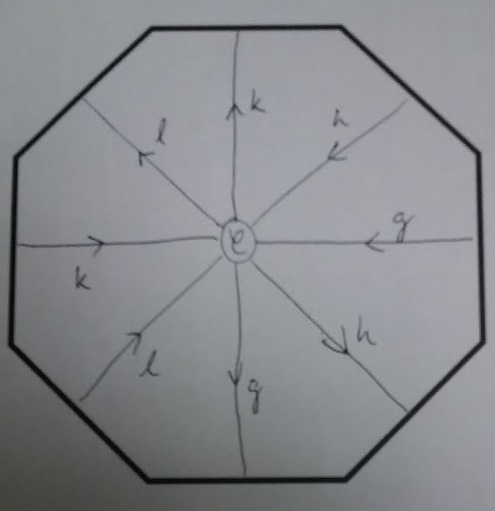
\includegraphics[width=0.5\textwidth]{basis.jpg}
\caption{Element of the spanning set $S$ for a genus 2 surface}
\label{fig:span}
\end{figure}

\begin{figure}
 \centering
 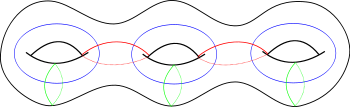
\includegraphics[width=.60\textwidth]{lickorish.png}
 \caption{Simple closed curves for the Dehn twists in the Lickorish generating set for the mapping class group of a genus $3$ closed surface. Reprinted from \cite{wiki:dt}.}
\label{fig:lickorish}
\end{figure}



The mapping class group of $\Si$ is generated by the Lickorish generating set consisting of Dehn twists around $3g-1$ simple closed curves.   These can be divided into two types of twists: the ones around a single hole (the blue and green curves in Figure \ref{fig:lickorish}), and the ones connecting two holes (the red curves). The action of a Dehn twist around a simple closed curve corresponds to cutting the manifold along the curve, holding one piece in place and twisting the other piece by $2\pi$ radians in a clockwise direction, then gluing the two pieces back together.


To understand the action of each type of Dehn twist on the representation space $H$, we will consider the action on the spanning set $S$.  First, we claim that we can apply local moves to any element of $S$ to get a colored graph of the form shown in the first subfigure of Figure \ref{fig:tikzTwist1_1}, where the unshown part of the fundamental polygon looks the same as in the definition of $S$.  Indeed, to pass from an arbitrary element of $S$, to a colored graph of the form shown in the first subfigure of $\ref{fig:tikzTwist1_1}$, we first add coevalution-labeled vertices to each  edge intersecting the three shown sides of the fundamental polygon.  Then connect the new vertices using edges labeled by the trivial object (this corresponds to applying the second local move in Figure \ref{f:local_rels1} with  $k = 0$), contract the connections to get one new vertex, and tensor together the edges connecting the old vertex to the new vertex.

The action of the first type of Dehn twist on an arbitrary element of $S$ is shown in the first two subfigures of Figure \ref{fig:tikzTwist1_1}.  
After applying the Dehn twist, we have the simple colored graph shown in the second subfigure of Figure \ref{fig:tikzTwist1_1}.  We then apply local moves in the remaining subfigures.  For example, to go from the second subfigure to the third, we first apply the third local move of Figure \ref{f:local_rels1} to add a $\coev$-labeled vertex to the top left $g$-labeled edge.  We then apply the second local move (tensoring edges) with the number of parallel edges $k = 0$ to add an edge labeled by the trivial object between the new vertex and the old one. To go from the third to the fourth subfigure, we apply the edge contraction local move on the new edge.  Lastly, we get to the fifth subfigure by applying the tensoring edges local move again (strictly speaking, this is not a valid move since it does not take place on a disk, but one can easily add a $\coev$-labeled vertex to each of the two parallel edges, connect them, contract the connection, tensor together each of the two pairs of parallel edges, and contract one of the resulting edges to get the same result). By repeated application of Proposition $\ref{prop:omega}$, the resulting colored graph is equivalent to $\beta \Delta$, for some $\beta \in \mu_{|G|}$ and  $\Delta \in S$.    Thus, the first type of Dehn twist maps $S$ to $\mu_{|G|} S$.

An analogous proof works for the second type of Dehn twist shown in Figure \ref{fig:tikzTwist2_0}. Thus, the image of any such mapping class group representation is a quotient of the group of permutations of the finite set $\mu_{|G|} S$, hence finite.
\end{proof}

\begin{rmk} 
When $\omega = 1$ and $\Si$ is closed, this representation is a permutation representation.  
\end{rmk}

\begin{proof}
Under the assumption that the representation in \cite{fjfu} coincides with ours, this fact follows from Theorem 2.6 in \cite{fjfu}, but we can also prove it directly.  We first note that $G$ acts on $S$ by simultaneous conjugation of all edge labels by a single element $g \in G$.  If $s \in S$ and $g \in G$, then we can retrieve $s$ from $gs$ by separating two oppositely oriented, $g$-labeled edges from each edge in the embedded graph $gs$.  This results in a loop labeled by $g$, whose evaluation is $1$.  Thus $gs$ is equivalent to $s$.  Moreover, the cardinality $|S/G| = |\Hom(\pi_1(M), G)|/|G|$ is equal to the dimension of the untwisted Dijkgraaf-Witten representation space $H$ \cite{dijkgraaf1990}.  Hence, $S/G$ is a basis for $H$.  The mapping class group action on $S$ commutes with the $G$-action, so the mapping class group permutes $S/G$, i.e. $H$ is a permutation representation.
\end{proof}

\newcommand{\nc}{\newcommand}
\newcommand{\rnc}{\renewcommand}

%% Definitions

    % boundary of polygon
    % top left corner
     \nc{\lcx}{-0.5}
     \nc{\lcy}{0.866}
     \nc{\rcx}{-\lcx}
     \nc{\rcy}{\lcy}

     %TODO: Color edges
     \nc{\makeBdy}{
       \begin{scope}[very thick,decoration={
             markings,
             mark=at position 0.5 with {\arrow{>}}}
         ]  

         \draw (-1,0) -- (\lcx, \lcy); 
         \draw (\lcx, \lcy) -- (\rcx, \rcy); 
         \draw  (1, 0) -- (\rcx, \rcy);
       \end{scope}
     }

    %cut    
    % left endpoint of cut
    \nc{\lcutx}{-0.6}
    \nc{\lcuty}{0.6928}
    \nc{\lcut}{(\lcutx, \lcuty)}
    \nc{\rcutx}{-\lcutx}
    \nc{\rcuty}{\lcuty}
    \nc{\rcut}{(\rcutx, \rcuty)}

    %Main vertex
    \nc{\mvx}{0}
    \nc{\mvy}{0.2}
    \nc{\mv}{(\mvx, \mvy)}

    % outgoing edge
    \nc{\outEdge}{\draw[postaction={decorate}]  (0, 0) -- \mv node[pos=.5, right]{$hgh^{-1}$};}

    % middle of top edge of polygon
    \nc{\mtopx}{0}
    \nc{\mtopy}{0.866}
    \nc{\mtop}{(\mtopx, \mtopy)}

\begin{figure}
\centering

\begin{tabular}{|c|c|}

\hline

%Dehn twist 1.1
    \begin{tikzpicture}[scale=3]    

      % boundary of polygon
      \makeBdy


    \begin{scope}[very thick,decoration={
    markings,
    mark=at position 0.5 with {\arrow{>}}}
    ]  

      % cut for Dehn twist
      \draw[loosely dashed] \lcut -- \rcut;
      

      %graph edges

      \draw[postaction={decorate}]   \mv -- (0.75, 0.433) node[pos=.5,sloped,above]{$h$};
      \draw[postaction={decorate}]   \mv -- \mtop node[pos=.5,left]{$g$};
      \draw[postaction={decorate}]  (-0.75, 0.433) -- \mv node[pos=.5,sloped,above]{$h$};
      \outEdge

    \end{scope}
    \end{tikzpicture}

&

%1.2
    \begin{tikzpicture}[scale=3]
    
    %boundary of polygon
      \makeBdy

    %graph edges
    \begin{scope}[very thick,decoration={
    markings,
    mark=at position 0.5 with {\arrow{>}}}
    ] 


        \draw[postaction={decorate}]   \mv -- (0.75, 0.433) node[pos=.5,sloped,above]{$h$};
        % old g
        % \draw[postaction={decorate}]   \rb -- (0, 0.866) node[pos=.5,left]{$g$};
        \draw[postaction={decorate}]  (-0.75, 0.433) -- \mv node[pos=.5,sloped,above]{$h$};
        \outEdge

        % new g
        \draw[postaction={decorate}]  \mv -- \rcut
        node[pos=.5,sloped,above]{$g$};
        \draw[postaction={decorate}]  \lcut -- \mtop
        node[pos=.5,sloped,below]{$g$};

    \end{scope}
    \end{tikzpicture}

\\ \hline

%1.3
      \begin{tikzpicture}[scale=3]
    
    %boundary of polygon
      \makeBdy

    %graph edges
    \begin{scope}[very thick,decoration={
    markings,
    mark=at position 0.5 with {\arrow{>}}}
    ] 

        \draw[postaction={decorate}]   \mv -- (0.75, 0.433) node[pos=.5,sloped,above]{$h$};
        \draw[postaction={decorate}]  (-0.75, 0.433) -- \mv node[pos=.5,sloped,above]{$h$};

        \outEdge

        \draw[postaction={decorate}]  \mv -- \rcut
        node[pos=.5,sloped,above]{$g$};
        %\draw[postaction={decorate}]  \lcut -- \mtop
        \draw[postaction={decorate}]  \lcut --  ({(\lcutx + \mtopx)/2} , {(\lcuty + \mtopy)/2})
        node[pos=.5,sloped,below]{$g$};
        \draw[postaction={decorate}]  ({(\lcutx + \mtopx)/2} , {(\lcuty + \mtopy)/2}) -- \mtop
        node[pos=.5,sloped,below]{$g$};


        \draw  \mv --  ({(\lcutx + \mtopx)/2} , {(\lcuty + \mtopy)/2});

    \end{scope}
    \end{tikzpicture}

&

%1.4
    
    \begin{tikzpicture}[scale=3]

      %boundary of polygon
      \makeBdy


      
      \begin{scope}[very thick,decoration={
            markings,
            mark=at position 0.5 with {\arrow{>}}}
        ] 
      %graph edges

        \draw[postaction={decorate}]   \mv -- (0.75, 0.433) node[pos=.5,sloped,above]{$h$};
        \draw[postaction={decorate}]  (-0.75, 0.433) -- \mv node[pos=.5,sloped,above]{$h$};

        \outEdge

        \draw[postaction={decorate}]  \mv -- \rcut
        node[pos=.5,sloped,above]{$g$};
        %\draw[postaction={decorate}]  \lcut -- \mtop
        \draw[postaction={decorate}]  \lcut -- \mv
        node[pos=.5,sloped,above]{$g$};
        \draw[postaction={decorate}]  \mv -- \mtop
        node[pos=.5,right]{$g$};


    \end{scope}
    \end{tikzpicture}

\\ \hline

%Dehn twist 1.5

    
    \begin{tikzpicture}[scale=3]

    % boundary of polygon
     \makeBdy
    
    %graph edges
    \begin{scope}[very thick,decoration={
    markings,
    mark=at position 0.5 with {\arrow{>}}}
    ]  
        \draw[postaction={decorate}]   \mv -- (0.75, 0.433) node[pos=.5,sloped,above]{$hg$};
        \draw[postaction={decorate}]   \mv -- \mtop node[pos=.5,left]{$g$};
        \draw[postaction={decorate}]  (-0.75, 0.433) -- \mv node[pos=.5,sloped,above]{$hg$};
        \outEdge

    \end{scope}
    \end{tikzpicture}

&

\\ \hline
\end{tabular}

\caption{Using local moves to calculate the action of the first type of Dehn twist on an arbitrary element of the spanning set $S$. Read from left to right, then top to bottom.  Unlabeled interior edges are colored by the group identity element.  The Dehn twist is performed along the dashed simple closed curve.  The first two subfigures show the action of the Dehn twist.  The last three show the local moves relating the image of the Dehn twist to another element of $S$.}
\label{fig:tikzTwist1_1}
\end{figure}

%%%%%%%%%%%% Twist 2 %%%%%%%%%%%%%%%%


\nc{\makeBdyTwo}{
  \begin{scope}[very thick,decoration={
    markings,
    mark=at position 0.5 with {\arrow{>}}}
    ]  
    \path[draw]
    (1.0,          0.0) --       %0
    (0.92388,      0.382683)  -- %1
    (0.707107,     0.707107) --  %2
    (0.382683,     0.92388) --   %3
    (0,            1.0)   --     %4
    (-0.382683,    0.92388) --   %5
    (-0.707107 ,   0.707107)  -- %6
    ( -0.92388,    0.382683) --  %7
    ( -1.0     ,   0);           %8

  \end{scope}
}


\nc{\mvTwo}{ (-0.312076, 0.753418) }

\nc{\outEdgeTwo}{\draw[postaction={decorate}]  (0, 0) -- \mv node[pos=.3, right]{$[a,b][c,d]$};}

% 0.9 1 + 0.1 6
\nc{\cutOneX}{{0.8*(-0.92388) + 0.2*(-0.707107)}}
\nc{\cutOneY}{{0.8*(0.382683) + 0.2*(0.707107)}}
\nc{\cutOne}{(\cutOneX, \cutOneY)}

%0.9 3 + 0.1 4
\nc{\cutTwoX}{{0.8*(0.382683) + 0.2*(0)}}
\nc{\cutTwoY}{{0.8*(0.92388) + 0.2*(1.0)}}
\nc{\cutTwo}{(\cutTwoX, \cutTwoY)}

%0.9 2 + 0.1 1
\nc{\cutThreeX}{{0.8*(0.707107 ) + 0.2*(0.92388 )}}
\nc{\cutThreeY}{{0.8*(0.707107 ) + 0.2*(0.382638 )}}
\nc{\cutThree}{(\cutThreeX, \cutThreeY)}

%0.9 2 + 0.1 3
\nc{\cutFourX}{{0.2*( 0.382683) + 0.8*(0.707107)}}
\nc{\cutFourY}{{0.2*( 0.92388) + 0.8*(0.707107)}}
\nc{\cutFour}{(\cutFourX, \cutFourY)}

%0.1 0   0.9 1
\nc{\cutFiveX}{{0.2*( 1.0) + 0.8*(0.92388)}}
\nc{\cutFiveY}{{0.2*( 0.0) + 0.8*(0.382638)}}
\nc{\cutFive}{(\cutFiveX, \cutFiveY)}

%0.1 2   0.9 1
\nc{\cutSixX}{{0.2*( 0.707107) + 0.8*(0.92388)}}
\nc{\cutSixY}{{0.2*( 0.707107) + 0.8*(0.382683)}}
\nc{\cutSix}{(\cutSixX, \cutSixY)}

%0.1 3      0.9 4
\nc{\cutSevenX}{{0.2*( 0.382683) + 0.8*(0.0)}}
\nc{\cutSevenY}{{0.2*( 0.92388) + 0.8*(1.0)}}
\nc{\cutSeven}{(\cutSevenX, \cutSevenY)}

%0.1 5 0.9 4
\nc{\cutEightX}{{0.2*( -0.382683) + 0.8*(0.0)}}
\nc{\cutEightY}{{0.2*( 0.92388) + 0.8*(1.0)}}
\nc{\cutEight}{(\cutEightX, \cutEightY)}

\begin{figure}
\centering

\begin{tabular}{|c|c|}

\hline
%2.1    
    \begin{tikzpicture}[scale=3]

    % boundary of polygon
     \makeBdyTwo

     % cut for Dehn twist
     \draw[dotted] \cutOne -- \cutTwo;
     \draw[dotted] \cutThree -- \cutFour;
     \draw[dotted] \cutFive -- \cutSix;
     \draw[dotted] \cutSeven -- \cutEight;
         
    %graph edges
    \begin{scope}[very thick,decoration={
    markings,
    mark=at position 0.5 with {\arrow{>}}}
    ]  
       \draw[postaction={decorate}]  \mv -- (   0.96194 , 0.191342) node[pos=.5,sloped,above]{$a$};
       \draw[postaction={decorate}]  \mv -- ( 0.815493,  0.544895) node[pos=.5,sloped,above]{$b$};
       \draw[postaction={decorate}] (0.544895,  0.815493) -- \mv  node[pos=.5,sloped,above]{$a$};
       \draw[postaction={decorate}]   (0.191342,  0.96194) -- \mv  node[pos=.4,sloped,above]{$b$}; 
       \draw[postaction={decorate}]  \mv -- (-0.191342,  0.96194) node[pos=.4,sloped,above]{$c$}; 
       \draw[postaction={decorate}]  \mv -- (-0.544895,  0.815493) node[pos=.5,sloped,above]{$d$}; 
       \draw[postaction={decorate}] (-0.815493,  0.544895) -- \mv  node[pos=.5,sloped,above]{$c$};
       \draw[postaction={decorate}] (-0.96194,   0.191342) -- \mv  node[pos=.5,sloped,above]{$d$};

         \outEdgeTwo
    \end{scope}
    \end{tikzpicture}

&

%2.2
    
    \begin{tikzpicture}[scale=3]

    % boundary of polygon
     \makeBdyTwo

     % cut for Dehn twist
     \draw[dotted] \cutOne -- \cutTwo;
     \draw[dotted] \cutThree -- \cutFour;
     \draw[dotted] \cutFive -- \cutSix;
     \draw[dotted] \cutSeven -- \cutEight;
         
    %graph edges
    \begin{scope}[very thick,decoration={
    markings,
    mark=at position 0.5 with {\arrow{>}}}
    ]  
       \draw[postaction={decorate}]  \mv -- \mvTwo node[pos=.5,sloped,above]{\tiny $g := b^{-1}cdc^{-1}$};

       \draw[postaction={decorate}]  \mv -- (   0.96194 , 0.191342) node[pos=.5,sloped,above]{$a$};
       \draw[postaction={decorate}]  \mv -- ( 0.815493,  0.544895) node[pos=.5,sloped,above]{$b$};
       \draw[postaction={decorate}] (0.544895,  0.815493) -- \mv  node[pos=.5,sloped,above]{$a$};
       \draw[postaction={decorate}]   (0.191342,  0.96194) -- \mvTwo  node[pos=.5,sloped,above]{$b$}; 
       \draw[postaction={decorate}]  \mvTwo -- (-0.191342,  0.96194) node[pos=.5,sloped,above]{$c$}; 
       \draw[postaction={decorate}]  \mvTwo -- (-0.544895,  0.815493) node[pos=.5,sloped,above]{$d$}; 
       \draw[postaction={decorate}] (-0.815493,  0.544895) -- \mvTwo  node[pos=.5,sloped,above]{$c$};
       \draw[postaction={decorate}] (-0.96194,   0.191342) -- \mv  node[pos=.5,sloped,above]{$d$};

         \outEdgeTwo
    \end{scope}
    \end{tikzpicture}

\\ \hline

%2.3
    
    \begin{tikzpicture}[scale=3]

    % boundary of polygon
     \makeBdyTwo
         
    %graph edges
    \begin{scope}[very thick,decoration={
    markings,
    mark=at position 0.5 with {\arrow{>}}}
    ]  
       \draw[postaction={decorate}]  \mv -- \cutTwo node[pos=.5,sloped,above]{$g$};
       \draw[postaction={decorate}]  \cutOne -- \mvTwo node[pos=.5,sloped,below]{$g$};
       \draw[postaction={decorate}]  \cutThree -- \cutFour node[pos=.5,sloped,below]{$g$};
       \draw[postaction={decorate}]  \cutFive -- \cutSix node[pos=.5,sloped,below]{$g$};
       \draw[postaction={decorate}]  \cutSeven -- \cutEight node[pos=.5,sloped,red]{$g$};


       \draw[postaction={decorate}]  \mv -- (   0.96194 , 0.191342) node[pos=.5,sloped,above]{$a$};
       \draw[postaction={decorate}]  \mv -- ( 0.815493,  0.544895) node[pos=.5,sloped,above]{$b$};
       \draw[postaction={decorate}] (0.544895,  0.815493) -- \mv  node[pos=.5,sloped,above]{$a$};
       \draw[postaction={decorate}]   (0.191342,  0.96194) -- \mvTwo  node[pos=.5,sloped,below]{$b$}; 
       \draw[postaction={decorate}]  \mvTwo -- (-0.191342,  0.96194) node[pos=.5,sloped,above]{$c$}; 
       \draw[postaction={decorate}]  \mvTwo -- (-0.544895,  0.815493) node[pos=.5,sloped,above]{$d$}; 
       \draw[postaction={decorate}] (-0.815493,  0.544895) -- \mvTwo  node[pos=.5,sloped,above]{$c$};
       \draw[postaction={decorate}] (-0.96194,   0.191342) -- \mv  node[pos=.5,sloped,above]{$d$};

         \outEdgeTwo
    \end{scope}
    \end{tikzpicture}

&

%2.4
    
    \begin{tikzpicture}[scale=3]

    % boundary of polygon
     \makeBdyTwo
         
    %graph edges
    \begin{scope}[very thick,decoration={
    markings,
    mark=at position 0.5 with {\arrow{>}}}
    ]  
       \draw[postaction={decorate}]  \mv -- \cutTwo node[pos=.5,sloped,above]{$g$};
       \draw[postaction={decorate}]  \cutThree -- \mv node[pos=.3,sloped,above]{$g$};

       \draw[postaction={decorate}]  \mv -- ( 0.96194 , 0.191342) node[pos=.8,sloped,above]{$ag^{-1}$};
       \draw[postaction={decorate}]  \mv -- ( 0.815493,  0.544895) node[pos=.7,sloped,below]{$gb$};
       \draw[postaction={decorate}] (0.544895,  0.815493) -- \mv  node[pos=.2,sloped,above]{$ag^{-1}$};
       \draw[postaction={decorate}]   (0.191342,  0.96194) -- \mvTwo  node[pos=.5,sloped,below]{$gb$}; 
       \draw[postaction={decorate}]  \mvTwo -- (-0.191342,  0.96194) node[pos=.5,sloped,above]{$gc$}; 
       \draw[postaction={decorate}]  \mvTwo -- (-0.544895,  0.815493) node[pos=.5,sloped,above]{$d$}; 
       \draw[postaction={decorate}] (-0.815493,  0.544895) -- \mvTwo  node[pos=.5,sloped,below]{$gc$};
       \draw[postaction={decorate}] (-0.96194,   0.191342) -- \mv  node[pos=.5,sloped,above]{$d$};

         \outEdgeTwo
    \end{scope}
    \end{tikzpicture}

\\ \hline 

%2.5

    \begin{tikzpicture}[scale=3]

    % boundary of polygon
     \makeBdyTwo
         
    %graph edges
    \begin{scope}[very thick,decoration={
    markings,
    mark=at position 0.5 with {\arrow{>}}}
    ]  
       \draw[postaction={decorate}]  \mv -- \cutTwo node[pos=.8,sloped,red]{$g$};
       \draw[postaction={decorate}]  \cutThree -- \mv node[pos=.2,sloped,above]{$g$};

       \draw[postaction={decorate}]  \mv -- ( 0.96194 , 0.191342) node[pos=.8,sloped,above]{$ag^{-1}$};
       \draw[postaction={decorate}]  \mv -- ( 0.815493,  0.544895) node[pos=.7,sloped,below]{$gb$};
       \draw[postaction={decorate}] (0.544895,  0.815493) -- \mv  node[pos=.2,sloped,above]{$ag^{-1}$};
       \draw[postaction={decorate}]   (0.191342,  0.96194) -- \mv  node[pos=.2,sloped,above]{$gb$}; 
       \draw[postaction={decorate}]  \mv -- (-0.191342,  0.96194) node[pos=.8,sloped,below]{$gc$}; 
       \draw[postaction={decorate}]  \mv -- (-0.544895,  0.815493) node[pos=.7,sloped,above]{$d$}; 
       \draw[postaction={decorate}] (-0.815493,  0.544895) -- \mv  node[pos=.3,sloped,above]{$gc$};
       \draw[postaction={decorate}] (-0.96194,   0.191342) -- \mv  node[pos=.3,sloped,above]{$d$};

         \outEdgeTwo
    \end{scope}
    \end{tikzpicture}

&

%2.6

    \begin{tikzpicture}[scale=3]

    % boundary of polygon
     \makeBdyTwo
         
    %graph edges
    \begin{scope}[very thick,decoration={
    markings,
    mark=at position 0.5 with {\arrow{>}}}
    ]  

       \draw[postaction={decorate}]  \mv -- ( 0.96194 , 0.191342) node[pos=.8,sloped,above]{$ag^{-1}$};
       \draw[postaction={decorate}]  \mv -- ( 0.815493,  0.544895) node[pos=.8,sloped,above]{$gbg^{-1}$};
       \draw[postaction={decorate}] (0.544895,  0.815493) -- \mv  node[pos=.2,sloped,above]{$ag^{-1}$};
       \draw[postaction={decorate}]   (0.191342,  0.96194) -- \mv  node[pos=.2,sloped,above]{$gbg^{-1}$}; 
       \draw[postaction={decorate}]  \mv -- (-0.191342,  0.96194) node[pos=.8,sloped,below]{$gc$}; 
       \draw[postaction={decorate}]  \mv -- (-0.544895,  0.815493) node[pos=.7,sloped,above]{$d$}; 
       \draw[postaction={decorate}] (-0.815493,  0.544895) -- \mv  node[pos=.3,sloped,above]{$gc$};
       \draw[postaction={decorate}] (-0.96194,   0.191342) -- \mv  node[pos=.3,sloped,above]{$d$};

         \outEdgeTwo
    \end{scope}
    \end{tikzpicture}

\\ \hline
\end{tabular}

\caption{Using local moves to calculate the action of the second type of Dehn twist on an arbitrary element of the spanning set $S$. Read from left to right, then top to bottom.   The Dehn twist is performed along the dashed simple closed curve.  The first two subfigures show application of local moves prior to the Dehn twist action. The third shows the action of the twist.  The last three show the local moves relating the image of the Dehn twist to another element of $S$.}
\label{fig:tikzTwist2_0}
\end{figure}


\section{Boundary Case}

When $\Si$ has boundary, we denote by $\MCG(\Si)$ the group of isotopy classes of homeomorphisms fixing the boundary of $\Si$ setwise. Given any labelling of the boundary  by objects in the Drinfeld center, $l : \pi_0(\partial M) \to \Obj(Z(\vgo))$, we get a mapping class group representation. The representation space is $\Hs(\Si, \VV)$ with boundary condition $\VV = F \circ l$, where $F$ is the forgetful functor $F: Z(\vgo) \to \vgo$.  The same local relations are valid in this representation space \cite{kirillovStringNets}.

By a similar argument as in the proof of the Theorem $\ref{thm:closed}$, any such representation space has a finite spanning set $S$ consisting of all simple colored graphs with a single vertex, loops for each of the usual generators of the fundamental group of $\Si$, and a leg from the vertex to each of the boundary components.  

Let $N$ denote the closed surface obtained by filling in all the boundary components of $\Si$ with disks. The mapping class group $\MCG(\Si)$ is generated by the same Dehn twists as $\MCG(N)$, as well as braids interchanging boundary components and mapping classes corresponding to dragging a boundary component along a representative of a standard generator of $\pi_1(N)$ \cite{birman}.  As in the proof of Theorem \ref{thm:closed}, applying any of these generators of $\MCG(\Si)$ to a colored graph in $S$ yields an element in $\mu_{|G|}S$ (see Figures \ref{fig:braid1} and \ref{fig:drag1}).  Since the braid group is also generated by such braids, we have the following theorem.


\nc{\rightX}{0.5}  % left marked point x value
\nc{\leftX}{-\rightX} % right marked point x value
\nc{\pY}{0.5}  % y value for marked points
\nc{\loopR}{0.3}
\renewcommand{\mv}{(0, -0.2)}

\nc{\makeBase}{
      % left loop
       \draw[very thick]  \mv -- ({\leftX - \loopR}, \pY);
       \draw[very thick]   ({\leftX + \loopR}, \pY) -- \mv;
       
       \begin{scope}[very thick,decoration={
             markings,
             mark=at position 0.5 with {\arrow{>}}}
         ]  

         % left leg
         \draw[postaction={decorate}]  \mv -- (\leftX, \pY) node[pos=.5,above]{$l$};

       \end{scope}

       % new right loop and leg
       \draw[very thick]  \mv -- ({\leftX - 4*\loopR}, \pY);
       \draw[very thick]   ({\leftX - 2*\loopR}, \pY) -- \mv;
 
       % right leg
       \draw[very thick]  \mv -- ({\leftX - 3*\loopR}, \pY);       

}


\nc{\makeBaseTwo}{
    % left loop

       \draw[very thick]   ({\leftX + \loopR}, \pY) -- \mv;
       
       \begin{scope}[very thick,decoration={
             markings,
             mark=at position 0.5 with {\arrow{>}}}
         ]  

         % left leg
         \draw[postaction={decorate}]  \mv -- (\leftX, \pY) node[pos=.5,above]{$l$};

       \end{scope}
  
       \draw[very thick]   ({\leftX - 2*\loopR}, \pY) -- \mv;
}


%bottom right of right loop
\nc{\bRight}{
        \begin{scope}[very thick,decoration={
           markings,
           mark=at position 0.5 with {\arrow{>}}}
       ]  
       \draw[postaction={decorate}]   plot[domain=360:180] ({\loopR*cos(\x) + \leftX + 3*\loopR}, {\loopR*sin(\x) + \pY});
       \node[below] at  ({\loopR*cos(270) + \leftX + 3*\loopR}, {\loopR*sin(270) + \pY}) {$g$};
     \end{scope}
   }

\nc{\makeBraid}{

     \makeBase

     \begin{scope}[very thick,decoration={
           markings,
           mark=at position 0.5 with {\arrow{>}}}
       ]  

       % left loop
       \draw[postaction={decorate}]   plot[domain=180:0]  
              ({\loopR*cos(\x) + \leftX}, {\loopR*sin(\x) + \pY});
       \node[above] at  ({\loopR*cos(90) + \leftX}, {\loopR*sin(90) + \pY}) {$k$};

       % right loop
       \draw[postaction={decorate}]     plot[domain=0:180] ({2*\loopR*cos(\x) + \leftX}, {2*\loopR*sin(\x) + \pY});
       \node[above] at  ({2*\loopR*cos(90) + \leftX}, {2*\loopR*sin(90) + \pY}) {$g$};
       \draw[postaction={decorate}]      plot[domain=180:0] ({4*\loopR*cos(\x) + \leftX}, {4*\loopR*sin(\x) + \pY});
       \node[above] at  ({4*\loopR*cos(90) + \leftX}, {4*\loopR*sin(90) + \pY}) {$g$};

       %\right leg
       \draw[postaction={decorate}]      plot[domain=180:0] ({3*\loopR*cos(\x) + \leftX}, {3*\loopR*sin(\x) + \pY});
       \node[above] at  ({3*\loopR*cos(90) + \leftX}, {3*\loopR*sin(90) + \pY}) {$h$};

     \end{scope}

     \bRight
       
}


\nc{\makeBraidOne}{

     \makeBase

     \begin{scope}[very thick,decoration={
           markings,
           mark=at position 0.25 with {\arrow{>}},
          mark=at position 0.75 with {\arrow{>}}}
       ]  

       % left loop
       \draw[postaction={decorate}]   plot[domain=180:0]  
              ({\loopR*cos(\x) + \leftX}, {\loopR*sin(\x) + \pY});
       \node[above] at  ({\loopR*cos(45) + \leftX}, {\loopR*sin(45) + \pY}) {$k$};
       \node[above] at  ({\loopR*cos(135) + \leftX}, {\loopR*sin(135) + \pY}) {$k$};

       % right loop
       \draw[postaction={decorate}]     plot[domain=0:180] ({2*\loopR*cos(\x) + \leftX}, {2*\loopR*sin(\x) + \pY});
       \node[above] at  ({2*\loopR*cos(45) + \leftX}, {2*\loopR*sin(45) + \pY}) {$g$};
       \node[above] at  ({2*\loopR*cos(135) + \leftX}, {2*\loopR*sin(135) + \pY}) {$g$};
       \draw[postaction={decorate}]      plot[domain=180:0] ({4*\loopR*cos(\x) + \leftX}, {4*\loopR*sin(\x) + \pY});
       \node[above] at  ({4*\loopR*cos(45) + \leftX}, {4*\loopR*sin(45) + \pY}) {$g$};
       \node[above] at  ({4*\loopR*cos(135) + \leftX}, {4*\loopR*sin(135) + \pY}) {$g$};

       %\right leg
       \draw[postaction={decorate}]      plot[domain=180:0] ({3*\loopR*cos(\x) + \leftX}, {3*\loopR*sin(\x) + \pY});
       \node[above] at  ({3*\loopR*cos(45) + \leftX}, {3*\loopR*sin(45) + \pY}) {$h$};
       \node[above] at  ({3*\loopR*cos(135) + \leftX}, {3*\loopR*sin(135) + \pY}) {$h$};

     \end{scope}

     \bRight       
}


\nc{\makeBraidTwo}{

     \makeBase


     \begin{scope}[very thick,decoration={
           markings,
           mark=at position 0.1 with {\arrow{>}},
          mark=at position 0.9 with {\arrow{>}}}
       ]  
       % \right leg
       \draw[postaction={decorate}]      plot[domain=180:0] ({3*\loopR*cos(\x) + \leftX}, {3*\loopR*sin(\x) + \pY});
       \node[right] at  ({3*\loopR*cos(18) + \leftX}, {3*\loopR*sin(18) + \pY}) {$h$};
       \node[left] at  ({3*\loopR*cos(162) + \leftX}, {3*\loopR*sin(162) + \pY}) {$h$};

       % left loop
       \draw[postaction={decorate}]      plot[domain=180:0] ({\loopR*cos(\x) + \leftX}, {3*\loopR*sin(\x) + \pY});
       \node[left] at  ({\loopR*cos(18) + \leftX}, {3*\loopR*sin(18) + \pY}) {$k$};
       \node[left] at  ({\loopR*cos(162) + \leftX}, {3*\loopR*sin(162) + \pY}) {$k$};
     \end{scope}

       % right loop
     \begin{scope}[very thick,decoration={
           markings,
           mark=at position 0.9 with {\arrow{>}}}]
       \draw[postaction={decorate}]         plot[domain=0:180] ({2*\loopR*cos(\x) + \leftX}, {3*\loopR*sin(\x) + \pY});
       \node[left] at  ({2*\loopR*cos(162) + \leftX}, {3*\loopR*sin(162) + \pY}) {$g$};
     \end{scope}
     \begin{scope}[very thick,decoration={
           markings,
           mark=at position 0.1 with {\arrow{>}}}]
     \draw[postaction={decorate}]       plot[domain=180:0] ({4*\loopR*cos(\x) + \leftX}, {3*\loopR*sin(\x) + \pY});
       \node[left] at  ({4*\loopR*cos(162) + \leftX}, {3*\loopR*sin(162) + \pY}) {$g$};
     \end{scope}
         
       \bRight
}

\nc{\makeBraidThree}{

  \makeBaseTwo

     \begin{scope}[very thick,decoration={
           markings,
          mark=at position 0.8 with {\arrow{>}}}
       ]  
       % \right leg
       \draw[postaction={decorate}]      plot[domain=90:0] ({3*\loopR*cos(\x) + \leftX}, {3*\loopR*sin(\x) + \pY});
       \node[right] at  ({3*\loopR*cos(18) + \leftX}, {3*\loopR*sin(18) + \pY}) {$h$};

       % left loop
       \draw[postaction={decorate}]      plot[domain=90:0] ({\loopR*cos(\x) + \leftX}, {3*\loopR*sin(\x) + \pY});
       \node[left] at  ({\loopR*cos(18) + \leftX}, {3*\loopR*sin(18) + \pY}) {$k$};
     \end{scope}

       % right loop
     \begin{scope}[very thick,decoration={
           markings,
           mark=at position 0.1 with {\arrow{>}}}]
       \draw[postaction={decorate}]         plot[domain=180:0] ({2*\loopR*cos(\x) + \leftX}, {3*\loopR*sin(\x) + \pY});
       \node[left] at  ({2*\loopR*cos(162) + \leftX}, {3*\loopR*sin(162) + \pY}) {$kg^{-1}hg$};
     \end{scope}

     \draw[very thick]       plot[domain=90:0] ({4*\loopR*cos(\x) + \leftX}, {3*\loopR*sin(\x) + \pY});
         
       \bRight
}


\begin{figure}
\centering

\begin{tabular}{|c|c|}

  \hline
  
  %Braid 1
    \begin{tikzpicture}[scale=2.5]

         
    %graph edges
    \begin{scope}[very thick,decoration={
    markings,
    mark=at position 0.5 with {\arrow{>}}}
    ]  


       % left loop
       \draw  \mv -- ({\leftX - \loopR}, \pY);
       \draw[postaction={decorate}]    plot[domain=180:0] ({\loopR*cos(\x) + \leftX}, {\loopR*sin(\x) + \pY});
       \node[above] at ({\loopR*cos(90) + \leftX}, {\loopR*sin(90) + \pY}) {$g$};
       \draw   ({\leftX + \loopR}, \pY) -- \mv;
       
       % left leg
       \draw[postaction={decorate}]  \mv -- (\leftX, \pY) node[pos=.5,above]{$h$};

       % right loop
       \draw  \mv -- ({\rightX - \loopR}, \pY);
       \draw[postaction={decorate}] plot[domain=180:0] ({\loopR*cos(\x) + \rightX}, {\loopR*sin(\x) + \pY});
       \node[above] at ({\loopR*cos(90) + \rightX}, {\loopR*sin(90) + \pY}) {$k$};
       \draw   ({\rightX + \loopR}, \pY) -- \mv;
 
       % right leg
       \draw[postaction={decorate}]  \mv -- (\rightX, \pY) node[pos=.5, above]{$l$};       
  
    \end{scope}
    \end{tikzpicture}

&

  %Braid 2
    \begin{tikzpicture}[scale=2.5]

         
    %graph edges
    \begin{scope}[very thick,decoration={
    markings,
    mark=at position 0.5 with {\arrow{>}}}
    ]  

    \makeBraid
  
    \end{scope}
    \end{tikzpicture}

\\ \hline

  %Braid 3
    \begin{tikzpicture}[scale=2.5]

      \makeBraidOne
         
    %graph edges
    \begin{scope}[very thick,decoration={
    markings,
    mark=at position 0.5 with {\arrow{>}}}
    ]  

       % connecting edge
       \draw ({\leftX}, {\pY + \loopR}) -- ({\leftX}, {\pY + 4*\loopR});
  
    \end{scope}
    \end{tikzpicture}

&

  %Braid 4
    \begin{tikzpicture}[scale=2.5]

      \makeBraidTwo     
         
    \end{tikzpicture}

\\ \hline

    %Braid 5
    \begin{tikzpicture}[scale=2.5]

      \makeBraidThree
         
    \end{tikzpicture}

&

  %Braid 6
    \begin{tikzpicture}[scale=2.5]

         
    %graph edges
    \begin{scope}[very thick,decoration={
    markings,
    mark=at position 0.5 with {\arrow{>}}}
    ]  


       % left loop
       \draw  \mv -- ({\leftX - \loopR}, \pY);
       \draw[postaction={decorate}]    plot[domain=180:0] ({\loopR*cos(\x) + \leftX}, {\loopR*sin(\x) + \pY});
       \node[above] at ({\loopR*cos(90) + \leftX}, {\loopR*sin(90) + \pY}) {$kg^{-1}hg$};
       \draw   ({\leftX + \loopR}, \pY) -- \mv;
       
       % left leg
       \draw[postaction={decorate}]  \mv -- (\leftX, \pY) node[pos=.5,above]{$l$};

       % right loop
       \draw  \mv -- ({\rightX - \loopR}, \pY);
       \draw[postaction={decorate}] plot[domain=180:0] ({\loopR*cos(\x) + \rightX}, {\loopR*sin(\x) + \pY});
       \node[above] at ({\loopR*cos(90) + \rightX}, {\loopR*sin(90) + \pY}) {$g$};
       \draw   ({\rightX + \loopR}, \pY) -- \mv;
 
       % right leg
       \draw[postaction={decorate}]  \mv -- (\rightX, \pY) node[pos=.5, above]{$h$};       
  
    \end{scope}
    \end{tikzpicture}

\\ \hline
\end{tabular}

\caption{Using local moves to calculate the action of a braid generator on an arbitrary element of the spanning set $S$. Read from left to right, then top to bottom.   Unlabeled interior edges are colored by the group identity element. The first two subfigures show application of the braid generator, which interchanges the univalent vertices. The last four show the local moves relating the image to another element of $S$.}
\label{fig:braid1}
\end{figure}


%%%%%%%%%%%%%%%%%% Dragging along \pi_1 generator %%%%%%%%%

\rnc{\mv}{(0,0)}
\nc{\uv}{(0, 0.7)}
\nc{\rvx}{0.3}
\nc{\rvy}{\lcuty}
\nc{\rv}{(\rvx, \rvy)}
\nc{\lv}{(-\rvx, \lcuty)}

\nc{\cutRatio}{0.5}
\rnc{\lcutx}{{\cutRatio*(-0.5) + (1-\cutRatio)*(-1)}}
\rnc{\lcuty}{{\cutRatio*(0.866)}}
\rnc{\lcut}{(\lcutx, \lcuty)}
\rnc{\rcutx}{{\cutRatio*(0.5) + (1-\cutRatio)*(1)}}
\rnc{\rcut}{(\rcutx, \lcuty)}
\nc{\boundaryComponentx}{0}
\nc{\boundaryComponenty}{\lcuty}
\nc{\boundaryComponent}{(\boundaryComponentx, \boundaryComponenty)}

\nc{\connectorEnd}{({0.5*(-0.85)}, {0.5*0.2598 + 0.5*0.433})}

\nc{\edgeRatio}{0.9}
\nc{\lex}{{\edgeRatio*(-1) + (1-\edgeRatio)*(\lcx)}}
\nc{\ley}{{(1-\edgeRatio)*(\lcy)}}
\nc{\lev}{(\lex, \ley)}
%\nc{\rex}{{(-1)*(\lex)}}
\nc{\rex}{{\edgeRatio*(1) + (1-\edgeRatio)*(\rcx)}}
\nc{\rev}{(\rex, \ley)}

\nc{\eOneRatio}{0.8}
\nc{\leOnex}{{\eOneRatio*(-1) + (1-\eOneRatio)*(\lcx)}}
\nc{\leOney}{{(1-\eOneRatio)*(\lcy)}}
\nc{\leOnev}{(\leOnex, \leOney)}
\nc{\reOnex}{{\eOneRatio*(1) + (1-\eOneRatio)*(\rcx)}}
\nc{\reOnev}{(\reOnex, \leOney)}

\nc{\eTwoRatio}{0.7}
\nc{\leTwox}{{\eTwoRatio*(-1) + (1-\eTwoRatio)*(\lcx)}}
\nc{\leTwoy}{{(1-\eTwoRatio)*(\lcy)}}
\nc{\leTwov}{(\leTwox, \leTwoy)}
\nc{\reTwox}{{\eTwoRatio*(1) + (1-\eTwoRatio)*(\rcx)}}
\nc{\reTwov}{(\reTwox, \leTwoy)}

\nc{\eThreeRatio}{0.6}
\nc{\leThreex}{{\eThreeRatio*(-1) + (1-\eThreeRatio)*(\lcx)}}
\nc{\leThreey}{{(1-\eThreeRatio)*(\lcy)}}
\nc{\leThreev}{(\leThreex, \leThreey)}
\nc{\reThreex}{{\eThreeRatio*(1) + (1-\eThreeRatio)*(\rcx)}}
\nc{\reThreev}{(\reThreex, \leThreey)}

\nc{\eFourRatio}{0.4}
\nc{\leFourx}{{\eFourRatio*(-1) + (1-\eFourRatio)*(\lcx)}}
\nc{\leFoury}{{(1-\eFourRatio)*(\lcy)}}
\nc{\leFourv}{(\leFourx, \leFoury)}
\nc{\reFourx}{{\eFourRatio*(1) + (1-\eFourRatio)*(\rcx)}}
\nc{\reFourv}{(\reFourx, \leFoury)}

\nc{\eFiveRatio}{0.2}
\nc{\leFivex}{{\eFiveRatio*(-1) + (1-\eFiveRatio)*(\lcx)}}
\nc{\leFivey}{{(1-\eFiveRatio)*(\lcy)}}
\nc{\leFivev}{(\leFivex, \leFivey)}
\nc{\reFivex}{{\eFiveRatio*(1) + (1-\eFiveRatio)*(\rcx)}}
\nc{\reFivev}{(\reFivex, \leFivey)}


\nc{\dby}{-0.2} %diagram bottom

\begin{figure}
\centering

\begin{tabular}{|c|c|}

  \hline
  
  % Drag 1
    \begin{tikzpicture}[scale=3]    

      % boundary of polygon
      \makeBdy


    \begin{scope}[very thick,decoration={
    markings,
    mark=at position 0.5 with {\arrow{>}}}
    ]  

      % cut for Dehn twist
      \draw[loosely dashed] \lcut -- \rcut;
      

      %graph edges
      \draw[postaction={decorate}]   (0, \dby) -- \mv node[pos=.5,right]{$p:=hglkl^{-1}h^{-1}$};
      \draw[postaction={decorate}]   \mv -- \rev node[pos=.5,sloped,above]{$h$};
      \draw[postaction={decorate}]   \mv -- \rv node[pos=.5,right]{$gl$};
      \draw[postaction={decorate}]   \mv -- \boundaryComponent node[pos=.5,left]{$k$};
      \draw[postaction={decorate}]   \lv -- \mv node[pos=.5,left]{$l$};
      \draw[postaction={decorate}]   \lev -- \mv node[pos=.5,sloped,below]{$h$};

      \draw[postaction={decorate}]   \rv -- \uv;
      \draw[postaction={decorate}]   \uv -- \mtop node[pos=.5,right]{$g$};
      \draw[postaction={decorate}]   \uv -- \lv;


    \end{scope}
    \end{tikzpicture}


&


  % Drag 2
    \begin{tikzpicture}[scale=3]    

      % boundary of polygon
      \makeBdy


    \begin{scope}[very thick,decoration={
    markings,
    mark=at position 0.5 with {\arrow{>}}}
    ]  


      %graph edges
      \draw[postaction={decorate}]   (0, \dby) -- \mv node[pos=.5,right]{$p$};
      \draw[postaction={decorate}]   \mv -- \rev node[pos=.5,sloped,below]{$h$};

      \draw[postaction={decorate}]   \mv -- \reOnev node[pos=.8,sloped,red]{$gl$};
      \draw[postaction={decorate}]   \leOnev -- \rv node[pos=.5,sloped,below]{$gl$};
      \draw[postaction={decorate}]   \rv -- \leFivev node[pos=.5,sloped,above]{$gl$};
      \draw[postaction={decorate}]   \reFivev -- \uv node[pos=.5,sloped,above]{$gl$};

      \draw[postaction={decorate}]   \mv -- \reTwov node[pos=.6,sloped,red]{$k$};
      \draw[postaction={decorate}]   \leTwov -- \boundaryComponent node[pos=.5,sloped,red]{$k$};

      \draw[postaction={decorate}]   \reThreev -- \mv node[pos=.5,sloped,above]{$l$};
      \draw[postaction={decorate}]   \lv -- \leThreev;
      \draw[postaction={decorate}]   \leFourv -- \lv node[pos=.5,sloped,above]{$l$};
      \draw[postaction={decorate}]   \uv -- \reFourv node[pos=.5,sloped,below]{$l$};

      \draw[postaction={decorate}]   \lev -- \mv node[pos=.5,sloped,below]{$h$};

      \draw[postaction={decorate}]   \uv -- \mtop node[pos=.5,right]{$g$};


    \end{scope}
    \end{tikzpicture}

\\ \hline


  % Drag 3
    \begin{tikzpicture}[scale=3]    

      % boundary of polygon
      \makeBdy

    \begin{scope}[very thick,decoration={
    markings,
    mark=at position 0.5 with {\arrow{>}}}
    ]  


      %graph edges
      \draw[postaction={decorate}]   (0, \dby) -- \mv node[pos=.5,right]{$p$};
      \draw[postaction={decorate}]   \mv -- \rev node[pos=.5,sloped,below]{$h$};

      \draw[postaction={decorate}]   \mv -- \reOnev node[pos=.8,sloped,red]{$gl$};
      \draw[postaction={decorate}]   \leOnev --  (-0.35, 0.3031) node[pos=.5,sloped,below]{$gl$};
      \draw[postaction={decorate}]   (-0.35, 0.3031) -- \rv node[pos=.5,sloped,below]{$gl$};

      \draw[postaction={decorate}]   \rv -- \leFivev node[pos=.5,sloped,above]{$gl$};
      \draw[postaction={decorate}]   \reFivev -- \uv node[pos=.5,sloped,above]{$gl$};

      \draw[postaction={decorate}]   \mv -- \reTwov node[pos=.6,sloped,red]{$k$};
      \draw[postaction={decorate}]   \leTwov -- \connectorEnd node[pos=.5,sloped,red]{$k$};
      \draw[postaction={decorate}]   \connectorEnd -- \boundaryComponent node[pos=.5,sloped,red]{$k$};


      \draw[postaction={decorate}]   \reThreev -- \mv node[pos=.5,sloped,above]{$l$};
      \draw[postaction={decorate}]   \lv -- \leThreev;
      \draw[postaction={decorate}]   \leFourv -- \lv node[pos=.5,sloped,above]{$l$};
      \draw[postaction={decorate}]   \uv -- \reFourv node[pos=.5,sloped,below]{$l$};

      \draw[postaction={decorate}]   \lev -- \mv node[pos=.5,sloped,below]{$h$};

      \draw[postaction={decorate}]   \uv -- \mtop node[pos=.5,right]{$g$};

      \draw \lcut -- \lv;
      \draw \rv -- \rcut;
      \draw \mv -- \connectorEnd;
     
    \end{scope}
    \end{tikzpicture}

&


  % Drag 4
    \begin{tikzpicture}[scale=3]    

      % boundary of polygon
      \makeBdy

    \begin{scope}[very thick,decoration={
    markings,
    mark=at position 0.5 with {\arrow{>}}}
    ]  


      %graph edges
      \draw[postaction={decorate}]   (0, \dby) -- \mv node[pos=.5,right]{$p$};
      \draw[postaction={decorate}]   \mv -- \rev node[pos=.5,sloped,below]{$h$};

      \draw[postaction={decorate}]   \mv -- \reOnev node[pos=.5,sloped,above]{$glk$};
      \draw[postaction={decorate}]   \leOnev --  (-0.35, 0.3031) node[pos=.5,sloped,above]{$glk$};
      \draw[postaction={decorate}]   (-0.35, 0.3031) -- \rv node[pos=.5,sloped,below]{$gl$};

      \draw[postaction={decorate}]   \rv -- \leFivev node[pos=.5,sloped,above]{$gl$};
      \draw[postaction={decorate}]   \reFivev -- \uv node[pos=.5,sloped,above]{$gl$};

      \draw[postaction={decorate}]    (-0.35, 0.3031)  -- \boundaryComponent node[pos=.5,sloped,above]{$k$};


      \draw[postaction={decorate}]   \rv -- \mv node[pos=.5,right]{$l$};
      \draw[postaction={decorate}]   \uv -- \rv node[pos=.5,right]{$l$};

      \draw[postaction={decorate}]   \lev -- \mv node[pos=.5,sloped,below]{$h$};

      \draw[postaction={decorate}]   \uv -- \mtop node[pos=.5,right]{$g$};


      \draw \mv --  (-0.35, 0.3031);
     
    \end{scope}
    \end{tikzpicture}


\\ \hline

  % Drag 5

 \begin{tikzpicture}[scale=3]    

      % boundary of polygon
      \makeBdy

    \begin{scope}[very thick,decoration={
    markings,
    mark=at position 0.5 with {\arrow{>}}}
    ]  


      %graph edges
      \draw[postaction={decorate}]   (0, \dby) -- \mv node[pos=.5,right]{$p$};
      \draw[postaction={decorate}]   \mv -- \rev node[pos=.5,sloped,below]{$hglk$};

      \draw[postaction={decorate}]   \rv -- \leFivev node[pos=.5,sloped,above]{$gl$};
      \draw[postaction={decorate}]   \reFivev -- \uv node[pos=.5,sloped,above]{$gl$};

      \draw[postaction={decorate}]    \mv  -- \boundaryComponent node[pos=.5,left]{$k$};


      \draw[postaction={decorate}]   \mv -- \rv node[pos=.5,right]{$l^{-1}gl$};
      \draw[postaction={decorate}]   \uv -- \rv node[pos=.5,right]{$l$};

      \draw[postaction={decorate}]   \lev -- \mv node[pos=.5,sloped,below]{$hglk$};

      \draw[postaction={decorate}]   \uv -- \mtop node[pos=.5,right]{$g$};
     
    \end{scope}
    \end{tikzpicture}

&


  % Drag 6

 \begin{tikzpicture}[scale=3]    

      % boundary of polygon
      \makeBdy

    \begin{scope}[very thick,decoration={
    markings,
    mark=at position 0.5 with {\arrow{>}}}
    ]  


      %graph edges
      \draw[postaction={decorate}]   (0, \dby) -- \mv node[pos=.5,right]{$p$};
      \draw[postaction={decorate}]   \mv -- \rev node[pos=.5,sloped,below]{$hglk$};

      \draw[postaction={decorate}]   \uv -- \leFivev node[pos=.5,sloped,below]{$gl$};
      \draw[postaction={decorate}]   \reFivev -- \uv node[pos=.5,sloped,below]{$gl$};

      \draw[postaction={decorate}]    \mv  -- \boundaryComponent node[pos=.5,left]{$k$};


      \draw[postaction={decorate}]   \mv -- \rv node[pos=.5,right]{$l^{-1}gl$};
      \draw[postaction={decorate}]   \rv -- \uv;

      \draw[postaction={decorate}]   \lev -- \mv node[pos=.5,sloped,below]{$hglk$};

      \draw[postaction={decorate}]   \uv -- \mtop node[pos=.5,right]{$g$};

     
    \end{scope}
    \end{tikzpicture}

\\ \hline

  % Drag 7

   \begin{tikzpicture}[scale=3]    

      % boundary of polygon
      \makeBdy

    \begin{scope}[very thick,decoration={
    markings,
    mark=at position 0.5 with {\arrow{>}}}
    ]  


      %graph edges
      \draw[postaction={decorate}]   (0, \dby) -- \mv node[pos=.5,right]{$p$};
      \draw[postaction={decorate}]   \mv -- \rev node[pos=.5,sloped,below]{$hglk$};

      \draw[postaction={decorate}]   \rev -- \uv node[pos=.5,sloped,above]{$gl$};
      \draw[postaction={decorate}]   \uv -- \lev node[pos=.5,sloped,above]{$gl$};

      \draw[postaction={decorate}]    \mv  -- \boundaryComponent node[pos=.5,left]{$k$};

      \draw[postaction={decorate}]   \mv -- \rv node[pos=.5,right]{$l^{-1}gl$};
      \draw[postaction={decorate}]   \rv -- \uv;

      \draw[postaction={decorate}]   \lev -- \mv node[pos=.5,sloped,below]{$hglk$};
      
      \draw[postaction={decorate}]   \uv -- \mtop node[pos=.5,right]{$g$};;

     
    \end{scope}
    \end{tikzpicture}

&

 % Drag 8
 \begin{tikzpicture}[scale=3]    

      % boundary of polygon
      \makeBdy

    \begin{scope}[very thick,decoration={
    markings,
    mark=at position 0.5 with {\arrow{>}}}
    ]  


      %graph edges
      \draw[postaction={decorate}]   (0, \dby) -- \mv node[pos=.5,right]{$p$};
      \draw[postaction={decorate}]   \mv -- \rev node[pos=.5,sloped,below]{$hglk$};

      \draw[postaction={decorate}]   \uv -- \leTwov  node[pos=.5,sloped,below]{$gl$};
      \draw[postaction={decorate}]   \reTwov -- \mv  node[pos=.5,sloped,above]{$gl$};

      \draw[postaction={decorate}]    \mv  -- \boundaryComponent node[pos=.5,left]{$k$};


      \draw[postaction={decorate}]   \mv -- \rv;
      \draw[postaction={decorate}]   \rv -- \uv node[pos=.5,right]{$g^2l$};

      \draw[postaction={decorate}]   \lev -- \mv node[pos=.5,sloped,below]{$hglk$};
      
      \draw[postaction={decorate}]   \uv -- \mtop node[pos=.5,right]{$g$};

     
    \end{scope}
    \end{tikzpicture}



\\ \hline


 % Drag 9
 \begin{tikzpicture}[scale=3]    

      % boundary of polygon
      \makeBdy

    \begin{scope}[very thick,decoration={
    markings,
    mark=at position 0.5 with {\arrow{>}}}
    ]  


      %graph edges
      \draw[postaction={decorate}]   (0, \dby) -- \mv node[pos=.5,right]{$p$};
      \draw[postaction={decorate}]   \mv -- \rev node[pos=.5,sloped,below]{$hglk$};

      \draw[postaction={decorate}]   \uv -- \leTwov node[pos=.5,sloped,below]{$gl$};
      \draw[postaction={decorate}]   \reTwov -- \mv node[pos=.5,sloped,above]{$gl$};
      \draw \leTwov -- \mv;

      \draw[postaction={decorate}]    \mv  -- \boundaryComponent node[pos=.5,left]{$k$};


      \draw[postaction={decorate}]   \mv -- \rv;
      \draw[postaction={decorate}]   \rv -- \uv node[pos=.5,right]{$g^2l$};

      \draw[postaction={decorate}]   \lev -- \mv node[pos=.5,sloped,below]{$hglk$};
      
      \draw[postaction={decorate}]   \uv -- \mtop node[pos=.5,right]{$g$};


     
    \end{scope}
    \end{tikzpicture}

&

% Drag 10

 \begin{tikzpicture}[scale=3]    

      % boundary of polygon
      \makeBdy

    \begin{scope}[very thick,decoration={
    markings,
    mark=at position 0.5 with {\arrow{>}}}
    ]  


      %graph edges
      \draw[postaction={decorate}]   (0, \dby) -- \mv node[pos=.5,right]{$p$};
      \draw[postaction={decorate}]   \mv -- \rev node[pos=.5,sloped,below]{$hglkl^{-1}g^{-1}$};

      \draw[postaction={decorate}]   \uv -- \lv;
      \draw[postaction={decorate}]   \lv -- \mv node[pos=.5,left]{$gl$};


      \draw[postaction={decorate}]    \mv  -- \boundaryComponent node[pos=.5,left]{$k$};


      \draw[postaction={decorate}]   \mv -- \rv;
      \draw[postaction={decorate}]   \rv -- \uv node[pos=.5,right]{$g^2l$};

      \draw[postaction={decorate}]   \lev -- \mv node[pos=.5,sloped,below]{$hglkl^{-1}g^{-1}$};
  
      \draw[postaction={decorate}]   \uv -- \mtop node[pos=.5,right]{$g$};


     
    \end{scope}
    \end{tikzpicture}


\\ \hline
\end{tabular}

\caption{Using local moves to calculate the action of the last Birman generator on an arbitrary element of the spanning set $S$.   This generator corresponds to pulling a boundary component of the surface $\Si$ along a generator for the fundamental group of the closed surface given by filling in all boundary components of $\Si$. Read from left to right, then top to bottom.   Unlabeled interior edges are colored by the group identity element. The first two figures show application of the Birman generator. The last eight show the local moves relating the image to another element of $S$.}

\label{fig:drag1}
\end{figure}


\begin{thrm}\label{thm:compact}
The image of any twisted Dijkgraaf-Witten representation of a mapping class group of an orientable, compact surface with boundary is finite.  In particular, the image of any such braid group representation is finite.
\end{thrm}


%% \section{Example Calculation}

%% This section contains a calculation of the coefficient for the first Dehn twist, shown in Table \ref{fig:tikzTwist1_1}.  WLOG we may assume that $\omega$ is normalized, i.e. that $\omega(1,x,y) = \omega(x,1,y) = \omega(x,y,1) = 1$ for all $x,y$.  We also assume that the main vertex is initially labeled with an element of $\Hom(\one, h \otimes g \otimes h^{-1} \otimes hg^{-1}h^{-1})$.   In the following, we will abbreviate this by saying that the vertex is in state $h \otimes g \otimes h^{-1} \otimes hg^{-1}h^{-1}$.

%% We add the upper left vertex, which is labeled by  $\coev_g$.  We then connect the vertices with an unlabelled edge, which is shorthand for labelling by the object $1$ .  At this point, the vertices are in states $h \otimes g \otimes 1 \otimes h^{-1} \otimes hg^{-1}h^{-1}$ and $g \otimes g^{-1}  \otimes 1$.  To compose the two vertices, we use the spherical structure on the former vertex and reassociate until it is in the state $h^{-1} \otimes h g^{-1} h^{-1} \otimes h \otimes g \otimes 1$.  In doing so, we pick up a factor of 
%% $$ \omega(h, g, h^{-1}) \omega(h, gh^{-1}, hg^{-1}h^{-1}) \omega(g, h^{-1}, hg^{-1}h^{-1}) \omega(g, g^{-1}h^{-1}, h) $$
%% % $$\omega^{-1}(hg^{-1}h^{-1}, hg, h^{-1}) \omega^{-1}(hg^{-1}h^{-1}, h, g) \omega^{-1}(h^{-1}, hg^{-1}, g) \omega^{-1}(h^{-1}, hg^{-1}h^{-1}, h) $$

%% After performing the composition, we are in state $h^{-1} \otimes hg^{-1}h^{-1} \otimes h \otimes g \otimes (g \otimes g^{-1})$.  To get rid of the last pair of parentheses, we get a factor of $\omega^{-1}(h^{-1}hg^{-1}h^{-1}hg, g, g^{-1}) = \omega^{-1}(1, g, g^{-1}) = 1$.   

%% To tensor the parallel $g$ and $h$ edges together, we add $\coev_g$ and $\coev_h$ vertices in the middle of those edges and connect them with a $1$.  Composing along the $1$, we get a vertex in state $g \otimes g^{-1} \otimes h^{-1} \otimes h$.  To put this vertex in state $g^{-1}h^{-1} \otimes hg$ we pick up a factor of $\omega(g, g^{-1}, h^{-1}) \omega(g, g^{-1}h^{-1}, h) \omega(g^{-1}h^{-1}, h, g)$.   We also put the original vertex in the state $g^{-1}h^{-1} \otimes hg^{-1}h^{-1} \otimes hg \otimes g$ with a factor of
%% $$\omega^{-1}(g^{-1}, g^{-1}, g) \omega^{-1}(g^{-1}, g^{-1}h^{-1}, h) \omega^{-1}(g^{-1}, h^{-1}, hg^{-1}h^{-1}) \omega(g^{-2}h^{-1}, h, g). $$

%% To compose the two vertices, we rotate the original vertex to the state $g  \otimes g^{-1}h^{-1}  \otimes hg^{-1}h^{-1} \otimes hg$ which yields a factor of 
%% $$\omega^{-1}(g, h^{-1}, hg) \omega^{-1}(g, g^{-1}h^{-1}, hg^{-1}h^{-1}) \omega^{-1}(g, g^{-1}, h^{-1}).$$
%% We are then in a position to compose the two vertices, giving a factor 
%% $\omega(g^{-1}h^{-1}, hg, g^{-1}h^{-1})  \ev_{g^{-1}h^{-1}} = 1$ and a vertex in state $g \otimes g^{-1}h^{-1} \otimes hg^{-1}h^{-1} \otimes hg$.  Rotating the vertex into its initial configuration $hg \otimes g \otimes  g^{-1}h^{-1} \otimes hg^{-1}h^{-1}$ gives a factor 
%% of 
%% $$\omega^{-1}(hg, h^{-1}, hg^{-1}h^{-1}) \omega^{-1}(hg, g, g^{-1}h^{-1}).$$

%%  Thus, we have an overall factor of
%% {\allowdisplaybreaks
%% \begin{align*} 
%% &  \frac{\omega(h, g, h^{-1}) \omega(h, gh^{-1}, hg^{-1}h^{-1}) \omega(g, h^{-1}, hg^{-1}h^{-1}) \omega(g, g^{-1}h^{-1}, h) } 
%% {\omega(g^{-1}, g^{-1}, g) \omega(g^{-1}, g^{-1}h^{-1}, h) \omega(g^{-1}, h^{-1}, hg^{-1}h^{-1})  \omega(g, g^{-2}h^{-1}, hg)} \cdot \\ 
%% & \qquad  \frac{\omega(g, g^{-1}, h^{-1}) \omega(g, g^{-1}h^{-1}, h) \omega(g^{-1}h^{-1}, h, g) \omega(g^{-2}h^{-1}, h, g)}
%% {\omega(g, g^{-1}h^{-1}, hg^{-1}h^{-1}) \omega(hg, h^{-1}, hg^{-1}h^{-1}) \omega(hg, g, g^{-1}h^{-1})} \\
%% & = \frac{\omega(h, g, g^{-1}h^{-1})\omega(g, g^{-1}h^{-1}, h) } 
%% {\omega(g^{-1}, g^{-1}, g) \omega(g^{-1}, g^{-1}h^{-1}, h) \omega(g^{-1}, h^{-1}, hg^{-1}h^{-1})  \omega(g, g^{-2}h^{-1}, hg)} \cdot \\ 
%% & \qquad \frac{\omega(g, g^{-1}, h^{-1}) \omega(g, g^{-1}h^{-1}, h) \omega(g^{-1}h^{-1}, h, g) \omega(g^{-2}h^{-1}, h, g)}
%% {\omega(g, g^{-1}h^{-1}, hg^{-1}h^{-1}) \omega(hg, g, g^{-1}h^{-1}) } \\
%% & = \frac{\omega(h, g, g^{-1}h^{-1})\omega(g, g^{-1}h^{-1}, h) } 
%% {\omega(g^{-1}, g^{-1}, g) \omega(g^{-1}, g^{-1}h^{-1}, h)  \omega(g, g^{-2}h^{-1}, hg)} \cdot \\ 
%% & \qquad \frac{\omega^2(g, g^{-1}, h^{-1}) \omega(g, g^{-1}h^{-1}, h) \omega(g^{-1}h^{-1}, h, g) \omega(g^{-2}h^{-1}, h, g)}
%% {\omega(g, g^{-1}, g^{-1}h^{-1}) \omega(hg, g, g^{-1}h^{-1}) } \\
%% & = \frac{\omega(h, g, g^{-1}h^{-1})\omega^2(g, g^{-1}h^{-1}, h) \omega^2(g, g^{-1}, h^{-1})  \omega^2(g^{-1}h^{-1}, h, g)} 
%% { \omega(g, g^{-2}h^{-1}, hg) \omega(g, g^{-1}, g^{-1}h^{-1}) \omega(hg, g, g^{-1}h^{-1}) \omega(g^{-1}, g^{-1}h^{-1}, hg)} \\
%% & = \frac{\omega(h, g, g^{-1}h^{-1})\omega^2(g, g^{-1}h^{-1}, h) \omega^2(g, g^{-1}, h^{-1}) \omega^2(g^{-1}h^{-1}, h, g) } 
%% {  \omega(hg, g, g^{-1}h^{-1}) } \\
%% & = \frac{\omega(h, g, g^{-1}h^{-1})  \omega^2(g^{-1}h^{-1}, h, g) } 
%% {\omega^2(g^{-1}, h^{-1},h)  \omega(hg, g, g^{-1}h^{-1}) } 
%% \end{align*}
%% }

